\section{System Overview}
Frequent incremental maintenance of materialized views can be costly or infeasible given system constraints such as throughput.
In our approach, we model this problem as a data cleaning problem.
Given an aggregation query (SUM, COUNT, AVG, VAR) on a stale materialized view, we use a sample of up-to-date (clean) data to estimate how much that data changes the stale aggregation query result.
The result is a correction term which adjusts or cleans the query result.

Our proposed system will work in conjunction with existing maintenance or re-calculation approaches.
We envision the scenario where materialized views are being refreshed periodically eg. nightly.
While maintaining the entire view throughout the day may be infeasible, sampling allows the database to scale maintenance with the performance and resource constraints during the day.
Then, between maintenance periods, we can provide approximately up-to-date query results for aggregation queries.

However, an additional challenge is that sampling has the potential mask outliers in the updates.
Since, we cannot answer selection queries on the view, we may miss outlier rows either because they were not sampled or because
they are averaged into an aggregation query.
We address this problem by using an ``outlier index" which is similar ones used in other works [?].
The ``outlier index" is an index on the base table which stores records with abnormal attribute values, where abnormality is defined by user specified ranges.
Therefore, we couple our sampling with outlier indexing to guarantee that rows in the materialized views derived outlier base table records are in the sample.
The result is that we can answer selection queries exactly on these outlier rows which are often the most queried rows in the materialized view.
What is particularly surprising is that outliers can give valuable information about the data distribution and these can be used to improve the accuracy of our aggregation queries as well.

\subsection{System Architecture}
The architecture of our proposed solution is shown in Figure \ref{sys-arch}.
The left side of the diagram resembles a typical materialized 
view maintenance architecture.
However, on the right side, there are a couple of key additions: (1) as updates arrive we sample the ``update pattern". 
(2) we maintain an outlier index, and (3) we combine the sample and the outlier index to process queries on the stale view.
In this section, we will introduce these three components, which are also explained in much more detail in the following sections.

\begin{figure}[h]
\label{sys-arch}
\centering
 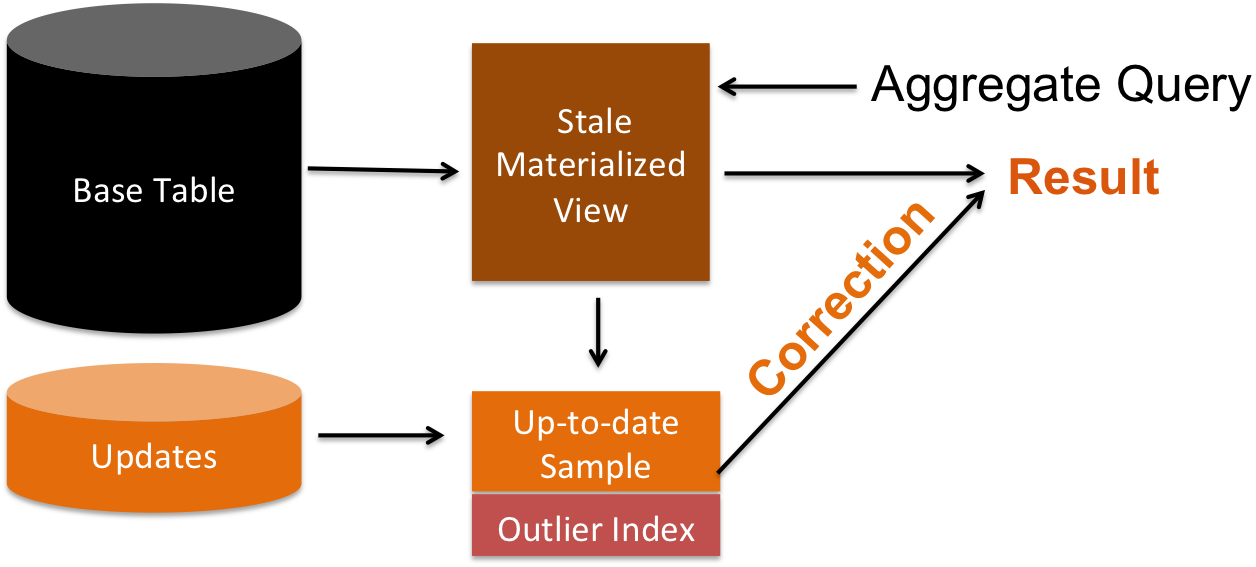
\includegraphics[width=\columnwidth]{figs/sys-arch.png}
 \caption{TODO}
\end{figure}

\subsubsection{Supported Materialized Views}\label{subsubsec:supported-view}
In this work, we bound aggregate queries (SUM, COUNT, AVG) on stale materialized views.
We will first introduce the taxonomy of materialized views that can benefit from our approach. 
\vspace{1em}

\noindent\textbf{Select-Project Views: } We can support all views that are derived from Select and Project operations. 

\vspace{1em}

\noindent\textbf{Foreign-Key Join Views: } As an extension to the Select-Project Views, we can support views derived from a Foreign-Key join. We can sample from the updates to any of the joined tables. Due to the Foreign-Key constraint, we ensure that sampling from the updates is sufficient to ensure the join can be executed. In this work, we do not consider all possible joins since for joins without Foreign-Keys they will, in general, have to scan the entire tables and not just the updates. Furthermore, many-to-one and one-to-many relationships change sampling statistics which complicates the query processing to calculate a correction.

\vspace{1em}

\noindent\textbf{Aggregation Views: } We also consider views derived from aggregate queries. These queries can have \textbf{WHERE} clause but we do not yet support queries with a \textbf{HAVING} clause.

\subsubsection{Sampling the Update Pattern}
Given these materialized views, the first challenge is sampling.
We have to sample the updates in a particular way so the sample accurately represents how updates
affect aggregation queries on the view. 
The three classes of views affect how we need to sample.
For example, insertions to the base database only result in insertions to Select-Project views but can result to updates to stale rows for Aggregation views.
In Section \ref{sampling}, we describe the sampling algorithm and a cost anylsis of how much sampling can reduce maintenance costs.

\subsubsection{Correcting a Query}
Once we have an appropriate sample, we can use information from the sample to correct stale query results.
Suppose, we issue an aggregate query to the stale view.
Then, we scan our sample, calculate an approximate correction.
The corrected result is in expectation up-to-date and is probabilistically bounded.
Like the sampling, the algorithm to calculate the correction varies between the types of views.
We detail query correction in Section \ref{correction}.

\subsubsection{Outlier Indexing}
We are often interested in records that outliers, 
which we define in this work as records with abnormally large attribute values.
Outliers and power-law distributions are a common property in web-scale datasets.
Often the queries of interest involve the outlier records, however sampling does 
have the potential to mask outliers in the updates.
If we have a small sampling ratio, more likely than not, outliers will be missed.

Therefore, we propose coupling sampling with outlier indexing. 
That is, we guarantee that records (or rows in the view derived from those records) 
with abnormally large attribute values are included in the sample.
What is particularly interesting is that these records give information about the distribution 
and can be used to reduce variance in our estimates.
See Section \label{outlier} for details on this component.


\subsubsection{Example Application: Log Analysis}
To illustrate our approach, we use the following running example which is a 
simplified schema of one of our experimental datasets (Figure \ref{example}).
Imagine, we are querying logs from a video streaming company. 
These logs record visits from users as they happen and grow over time.
We have two table: Log and Video, with the following schema:
\begin{lstlisting}
Log(sessionID, videoID, responseTime, userAgent)
Video(videoID, title, duration)
\end{lstlisting}
These tables are related with a foreign-key relationship between
Log and Video, and there is an integrity constraint that every log
record must link to one video in the video table.

\begin{figure}[h]
\label{example}
\centering
 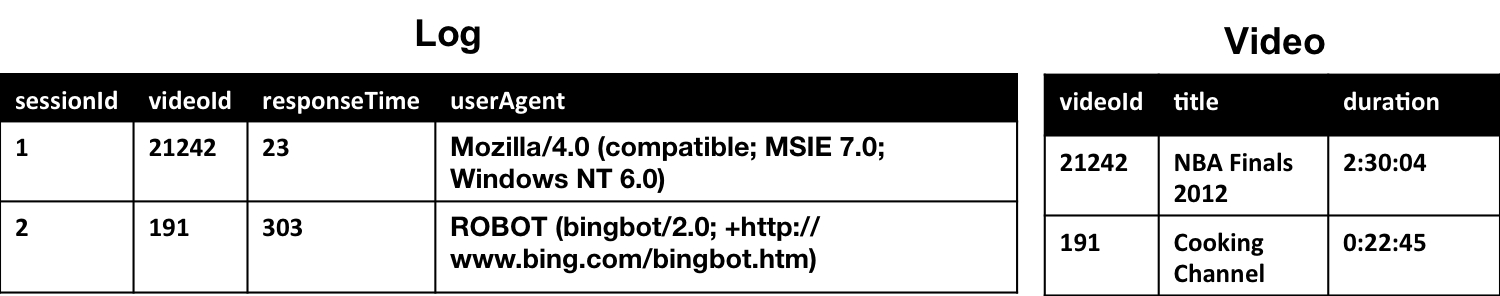
\includegraphics[width=\columnwidth]{figs/sample-clean-example.png}
 \caption{TODO}
\end{figure}

Consider the following example materialized view \textbf{AggView}, which stores a result for each video and the maximum time it took for the server to load that video:
\begin{lstlisting} 
SELECT videoID, 
max(responseTime) AS maxResponseTime 
FROM Log 
GROUP BY videoID;
\end{lstlisting}

Suppose, the user creates and materializes this view.
The user wants to know how many videos had a max response time of greater than 100ms.
\begin{lstlisting} 
SELECT COUNT(1)
FROM AggView
WHERE maxResponseTime > 100
\end{lstlisting}
Let us suppose the query result is $15$.

Now, there have been new logs records inserted into to the Log table. 
So materialized aggregation view and the old result of $15$ are now stale.
For example, if our sampling ratio 5\%, our system maintains a sample of this view.
That means for 5\% of the videos (distinct videoID's) we refresh stale maxResponseTime if necessary.
From this sample, we calculate how many new videos changed from a maxResponseTime of less than 100ms to times greater than 100ms; let us suppose this answer is $2$.
Since our sampling ratio is 5\%, we extrapolate that $10$ new videos throughout the view should now be included in the count, resulting in the estimate of $25$.
In contrast, if we had applied SAQP, we would have counted how many videos in the sample had a max response time of greater than 100ms.
In our experiments (Section \ref{exp}), we show that our correction approach compared to SAQP is more accurate when number of updated rows is small compared to the total size of the materialized view.